\documentclass[10pt,a4paper]{article}

\usepackage[utf8]{inputenc}
\usepackage{a4wide}
\usepackage{amsmath,amssymb}
\usepackage{boxproof}
\usepackage{daymonthyear}
\usepackage{enumerate}
\usepackage{float} % for the H placement identifier
\usepackage{listings}
\usepackage{multicol}
\usepackage{stmaryrd}
\usepackage{tikz}

%========== DEFINITIONS ==========%

\definecolor{c_comment}{rgb}	{0.38, 0.62, 0.38}
\definecolor{c_keyword}{rgb}	{0.10, 0.10, 0.81}
\definecolor{c_identifier}{rgb}	{0.00, 0.00, 0.00}
\definecolor{c_string}{rgb}		{0.50, 0.50, 0.50}

%===== SETTINGS =====%

\lstset
{
	numbers=left,
	frame=single,
	basicstyle=\footnotesize\ttfamily,
	tabsize=4,
	% colors
	commentstyle=\color{c_comment},
	keywordstyle=\color{c_keyword},
	identifierstyle=\color{c_identifier},
	stringstyle=\color{c_string},
}

\def\meta#1{\mbox{$\langle\hbox{#1}\rangle$}}
\def\macrowitharg#1#2{{\tt\string#1\bra\meta{#2}\ket}}

{\escapechar-1 \xdef\bra{\string\{}\xdef\ket{\string\}}}

\def\intro#1{{#1}{\cal I}}
\def\elim#1{{#1}{\cal E}}

\showboxbreadth 999
\showboxdepth 999
\tracingoutput 1

\let\imp\to
\def\elim#1{{{#1}{\cal E}}}
\def\intro#1{{{#1}{\cal I}}}
\def\lt{<}
\def\eqdef{\overset{\mathrm{def}}{=\joinrel=}}
\def\eps{\mathrel{\epsilon}}
\def\biimplies{\leftrightarrow}
\def\flt#1{\mathrel{{#1}^\flat}}
\def\setof#1{{\left\{{#1}\right\}}}
\let\implies\to
\def\KK{{\mathsf K}}
\let\squashmuskip\relax

%===== META DATA =====%

\title
{
	{\Large Logic in Computer Science}\\
	Exam
}
\author
{
	Casper B. Hansen\\
	University of Copenhagen\\
	Department of Computer Science\\
	{\tt fvx507@alumni.ku.dk}
}
\date{\today}

%===== DOCUMENT =====%

\begin{document}

\maketitle

\section{Propositional logic}
\subsection*{Question 1.1}
This subquestion concerns the use of {\it proof theoretic} argument in
propositional logic, i.e. arguments relating to natural deduction. Note that
you may {\it only} use the rules of page 27 in Huth+Ryan. You are not allowed
to shortcut your formal proofs with equivalences.
\subsubsection*{(a) \mdseries Use natural deduction for propositional logic
(i.e. the deduction system on page 27 of Huth+Ryan) to show that the following
sequents are valid.}

\begin{enumerate}[i]
	\item
	{
	$\vdash \neg\neg p \land q \imp p \lor r$
	\begin{proofbox}
	\[
		\lbl{1} \: \neg\neg p \land q 			\=\mbox{assumption} \\
		\lbl{2} \: \neg\neg p 					\=\elim\land_1(\ref{1}) \\
		\lbl{3} \: q 							\=\elim\land_2(\ref{1}) \\
		\lbl{4} \: p 							\=\elim{\neg\neg}(\ref{2}) \\
	\(
		\lbl{5} \: p 							\=\mbox{assumption} \\
		\lbl{6} \: p \lor r						\=\intro\lor_1(\ref{5}) \\
	\*
		\lbl{5} \: r							\=\mbox{assumption} \\
		\lbl{6} \: p \lor r						\=\intro\lor_2(\ref{5}) \\
	\)
		\lbl{7} \: p \lor r 					\=\elim\lor(1, 5-6, 5-6) \\
	\]
		\lbl{8} \: (\neg\neg p \land q) \imp p \lor r 	\=\intro\imp(1-7) \\
	\end{proofbox}
	}
	\item
	{
	$\neg q \imp \neg p \vdash p \imp q$
	\begin{proofbox}
		\lbl{1} \: \neg q \imp \neg p 			\=\mbox{premise} \\
	\[
		\lbl{2} \: p 							\=\mbox{assumption} \\
	\[
		\lbl{3} \: \neg q 						\=\mbox{assumption} \\
		\lbl{4} \: \neg p 					\=\elim\imp(\ref{1}, \ref{3}) \\
		\lbl{5} \: \bot 					\=\elim\neg(\ref{2}, \ref{4}) \\
	\]
		\lbl{6} \: \neg\neg q 					\=\intro\neg(3-5) \\
		\lbl{7} \: q 							\=\elim{\neg\neg}(\ref{6}) \\
	\]
		\lbl{8} \: p \imp q 					\=\intro\imp(2, 7) \\
	\end{proofbox}
	}
\end{enumerate}

\subsubsection*{(b) \mdseries A deduction rule (without boxes) of form
\[\frac{\phi_1\quad\phi_2\quad\dots\quad\phi_n}{\psi}\text{\scriptsize R}\] is
called {\it derivable} if the conclusion $\psi$ can be derived from the
premises $\phi_1,\dots,\phi_n$ without using rule R. In other words, if you
can provide a proof schema for $\phi_1,\phi_2,\dots,\phi_n\vdash\psi$, using
just the rules of natural deduction for propositional logic, then rule R is
derivable.
\newline\indent
As an example, the rule \[\frac{\phi\imp\neg\phi}{\neg\phi}\text{\scriptsize NREL}\] is
derivable by the proof schema
\begin{proofbox}
	\lbl{1}	\: \phi \imp \neg\phi 				\=\mbox{premise} \\
\[
	\lbl{2}	\: \phi 							\=\mbox{assumption} \\
	\lbl{3}	\: \neg\phi 					\=\elim\imp(\ref{1}, \ref{2}) \\
	\lbl{4}	\: \bot 						\=\elim\neg(\ref{2}, \ref{3}) \\
\]
	\lbl{5}	\: \neg\phi 						\=\intro\neg(2, 4) \\
\end{proofbox}
Show that the following rules are derivable.}

\begin{enumerate}[i]
	\item
	{
	$\frac{\phi}{\psi \imp \phi}\text{\scriptsize WEAK}$
	\begin{proofbox}
		\lbl{1} \: \phi 					\=\mbox{premise} \\
	\[
		\lbl{2} \: \psi 					\=\mbox{assumption} \\
		\lbl{3} \: \phi 					\=\mbox{copy(\ref{1})} \\
	\]
		\lbl{4} \: \psi \imp \phi 			\=\intro\imp(2-3) \\
	\end{proofbox}
	}
	\item
	{
	$\frac{\phi \lor \psi \quad \neg\psi}{\phi}\text{\scriptsize EXT}$
	\begin{proofbox}
		\lbl{1} \: \phi \lor \psi 				\=\mbox{premise} \\
		\lbl{2} \: \neg\psi 					\=\mbox{premise} \\
	\(
		\lbl{3} \: \phi 						\=\mbox{assumption} \\
	\*
		\lbl{3} \: \psi 						\=\mbox{assumption} \\
		\lbl{4} \: \bot 						\=\elim\neg(\ref{2},\ref{3}) \\
		\lbl{5} \: \phi 						\=\elim\bot(\ref{4}) \\
	\)
		\lbl{6} \: \phi 						\=\elim\lor(3-5) \\
	\end{proofbox}
	}
\end{enumerate}

\newpage
\subsection*{Question 1.2}
This subquestion concerns the use of {\it semantic} arguments in propositional
logic, i.e. argument that have to do with truth tables and valuations, in some
way.

\subsubsection*{(a) \mdseries For the following formulas, decide whether they
are {\it satisfiable} or not, and whether they are {\it valid} or not. Justify
your answer.}
\begin{enumerate}[i]
	\item
	{
	$(\neg p \imp q \land r) \land (\neg (q \land r) \imp p)$ \\\\
	We give the truth table for all valuations of the formula above. \\\\
	\begin{tabular}{ccccccc|c}
		$p$ & $q$ & $r$ &
		$q \land r$ &
		$\neg (q \land r)$ &
		$\neg p \imp q \land r$ &
		$\neg (q \land r) \imp p$ &
		$(\neg p \imp q \land r) \land (\neg (q \land r) \imp p)$ \\ \hline
		{\tt F} & {\tt F} & {\tt F} & {\tt F} & {\tt T} & {\tt T} & {\tt F} & {\tt F} \\
		{\tt F} & {\tt F} & {\tt T} & {\tt F} & {\tt T} & {\tt T} & {\tt F} & {\tt F} \\
		{\tt F} & {\tt T} & {\tt F} & {\tt F} & {\tt T} & {\tt T} & {\tt F} & {\tt F} \\
		{\tt F} & {\tt T} & {\tt T} & {\tt T} & {\tt F} & {\tt T} & {\tt T} & {\tt T} \\
		{\tt T} & {\tt F} & {\tt F} & {\tt F} & {\tt T} & {\tt F} & {\tt T} & {\tt F} \\
		{\tt T} & {\tt F} & {\tt T} & {\tt F} & {\tt T} & {\tt F} & {\tt T} & {\tt F} \\
		{\tt T} & {\tt T} & {\tt F} & {\tt F} & {\tt T} & {\tt F} & {\tt T} & {\tt F} \\
		{\tt T} & {\tt T} & {\tt T} & {\tt T} & {\tt F} & {\tt T} & {\tt T} & {\tt T} \\
	\end{tabular} \\\\
	The formula is satisfiable, since at least one valuation of the formulas
	constituent propositional atoms produce a true statement --- in this case
	we have two. By definition 1.34\cite{HR}, we have that when all the
	propositional atoms $p$, $q$ and $r$ are {\tt T}, so is the formula, and
	hence $\models (\neg p \imp q \land r) \land (\neg (q \land r) \imp p)$.
	}
	
	\item
	{
	$p \lor (p \imp p \lor r) \lor (\neg p \land (q \lor r))$ \\\\
	We give the truth table for all valuations of the formula above. \\\\
	\begin{tabular}{cccccc|c}
		$p$ & $q$ & $r$ &
		$q \lor r$ &
		$p \lor (p \imp p \lor r)$ &
		$\neg p \land (q \lor r)$ &
		$p \lor (p \imp p \lor r) \lor (\neg p \land (q \lor r))$ \\ \hline
		{\tt F} & {\tt F} & {\tt F} & {\tt F} & {\tt T} & {\tt F} & {\tt T} \\
		{\tt F} & {\tt F} & {\tt T} & {\tt T} & {\tt T} & {\tt T} & {\tt T} \\
		{\tt F} & {\tt T} & {\tt F} & {\tt T} & {\tt T} & {\tt T} & {\tt T} \\
		{\tt F} & {\tt T} & {\tt T} & {\tt T} & {\tt T} & {\tt T} & {\tt T} \\
		{\tt T} & {\tt F} & {\tt F} & {\tt F} & {\tt T} & {\tt F} & {\tt T} \\
		{\tt T} & {\tt F} & {\tt T} & {\tt T} & {\tt T} & {\tt F} & {\tt T} \\
		{\tt T} & {\tt T} & {\tt F} & {\tt T} & {\tt T} & {\tt F} & {\tt T} \\
		{\tt T} & {\tt T} & {\tt T} & {\tt T} & {\tt T} & {\tt F} & {\tt T} \\
	\end{tabular} \\\\
	The formula is satisfiable, since at least one valuation of the formulas
	constituent propositional atoms produce a true statement --- in this case
	all valuations produce a true statement. By definition 1.34\cite{HR}, it
	is trivial to see that since all valuations makes the formula true, so
	follows the semantic entailment. That is, we have that $\models p \lor
	(p \imp p \lor r) \lor (\neg p \land (q \lor r))$.
	}
\end{enumerate}

\newpage
\subsubsection*{(b) \mdseries Show that \[\models \left((\phi_1 \land \phi_2
\land \dots \land \phi_n) \imp \psi \right) \imp \left( (\phi_1 \imp \psi)
\land (\phi_2 \imp \psi) \land \dots \land (\phi_n \imp \psi) \right)\] does
{\it not} hold in general, by exhibiting a concrete counterexample formula
$\phi$ and valuation $\cal L$ showing $\phi$ is not valid.} 
Suppose that the implication does not hold, then there exists a valuation,
for which it evaluates to {\tt false}. For this to happen, we must have that
the left-hand side of the expression ($(\phi_1 \land \dots \land \phi_n) \imp
\psi$) evaluates to {\tt T}, while the right-hand side $(\phi_1 \imp \psi)
\land \dots \land (\phi_n \imp \psi)$ must evaluate to {\tt F}.

\begin{itemize}
	\item For the left-hand side, at least one of its constituents $\phi$ must be
{\tt F}. We choose $\phi_i$ to be {\tt F}.

	\item For the right-hand side, chosing $\psi$ to be {\tt F} and another constituent
$\phi_j$ to be {\tt T} makes it so.
\end{itemize}

\noindent We arrive at a formula $\phi$ that reads
\scriptsize
\begin{align*}
	\star = 
	(
		(\phi_1 \land \dots \land \phi_i \land \dots \land \phi_j \land \dots \land \phi_n) \imp \psi
	)
	\imp
	(
		(\phi_1 \imp \psi) \land \dots \land
		(\phi_i \imp \psi) \land \dots \land
		(\phi_j \imp \psi) \land \dots \land
		(\phi_n \imp \psi)
	)
\end{align*}
\normalsize
For which the truth table entries of interest reveals that it does not hold.

\begin{tabular}{ccc|c|c|c}
	$\phi_i$ & $\phi_j$ & $\psi$
	& $(\phi_1 \land \dots \land \phi_n) \imp \psi$
	& $(\phi_1 \imp \psi) \land \dots \land (\phi_n \imp \psi)$
	& $\star$ \\ \hline
	{\tt F} & {\tt T} & {\tt F} & {\tt T} & {\tt F} & {\tt F} \\
	{\tt T} & {\tt F} & {\tt F} & {\tt T} & {\tt F} & {\tt F} \\
\end{tabular}

\section{The SAT solver}
\subsection*{Question 2.1}
\subsubsection*{(a) \mdseries ...}
Using the grammar, as defined on $\phi$, we write up the structural induction.
\begin{enumerate}
	\item $T(p) \models p$ and $T(\neg p) \models \neg p$
	\item $T(\neg \phi) \models \neg (T(\phi))$
	\item $T(\phi_1 \land \phi_1) \models T(\phi_1) \land T(\phi_2)$
	iff. $\models \phi_1$ and $\models \phi_2$
	\item $T(\phi_1 \uparrow \phi_1) \models \neg(\phi_1 \land \phi_2)$
	iff. $\models \neg \phi_1$ and $\models \neg \phi_2$
\end{enumerate}
By the structural induction above, we see that $\phi \equiv T(\phi)$. Also,
no conditions need be satisfied for $T(\cdot)$ to hold in which $\uparrow$
occurs. Hence $T(\phi)$ does not contain the $\uparrow$ as a connective.

\subsubsection*{(b) \mdseries ...}

\subsection*{Question 2.2}
\subsubsection*{(a) \mdseries Create {\it forcing rules} for $\uparrow$.}
\usetikzlibrary{arrows}
\begin{figure}[H]
	\center
	\begin{multicols}{3}
	\begin{tikzpicture}
	[
	align=center,
	node/.style={},
	]
		% connective
		\node[node] (cv) at 		( 0.0,  0.0 ) {\tt F};
		\node[node] (cs) at 		( 0.0, -0.5 ) {$\uparrow$};
		
		% left-hand side
		\node[node] (lv) at 		(-1.0, -1.0 ) {\tt T};
		\node[node] (ls) at 		(-1.0, -1.5 ) {$\circ$};
		
		% right-hand side
		\node[node] (rv) at 		( 1.0, -1.0 ) {\tt T};
		\node[node] (rs) at 		( 1.0, -1.5 ) {$\circ$};
		
		\foreach \from/\to in {cs/ls,cs/rs} \draw[solid] (\from) -- (\to);
		% \foreach \from/\to in {cv/lv,cv/rv} \draw[double] (\from) -- (\to);
		
	\end{tikzpicture}\\
	When the connective node is {\tt F}, it forces both subnodes to become
	{\tt T}.
	
	\vfill
	\columnbreak
	
	\begin{tikzpicture}
	[
	align=center,
	node/.style={},
	]
		% connective
		\node[node] (cv) at 		( 0.0,  0.0 ) {\tt T};
		\node[node] (cs) at 		( 0.0, -0.5 ) {$\uparrow$};
		
		% left-hand side
		\node[node] (lv) at 		(-1.0, -1.0 ) {\tt F};
		\node[node] (ls) at 		(-1.0, -1.5 ) {$\circ$};
		
		% right-hand side
	%	\node[node] (rv) at 		( 1.0, -1.0 ) {\tt F};
		\node[node] (rs) at 		( 1.0, -1.5 ) {$\circ$};
		
		\foreach \from/\to in {cs/ls,cs/rs} \draw[solid] (\from) -- (\to);
	%	\foreach \from/\to in {cv/lv,cv/rv} \draw[double] (\from) -- (\to);
		
	\end{tikzpicture}\\
	If either of the connectives subnodes are {\tt F}, it then forces the
	node to become {\tt T}.
	
	\vfill
	\columnbreak
	
	\begin{tikzpicture}
	[
	align=center,
	node/.style={},
	]
		% connective
		\node[node] (cv) at 		( 0.0,  0.0 ) {\tt T};
		\node[node] (cs) at 		( 0.0, -0.5 ) {$\uparrow$};
		
		% left-hand side
		\node[node] (lv) at 		(-1.0, -1.0 ) {\tt T};
		\node[node] (ls) at 		(-1.0, -1.5 ) {$\circ$};
		
		% right-hand side
		\node[node] (rv) at 		( 1.0, -1.0 ) {\tt F};
		\node[node] (rs) at 		( 1.0, -1.5 ) {$\circ$};
		
		\foreach \from/\to in {cs/ls,cs/rs} \draw[solid] (\from) -- (\to);
	%	\foreach \from/\to in {cv/lv,cv/rv} \draw[double] (\from) -- (\to);
		
	\end{tikzpicture}\\
	If we know the connective node to be {\tt T}, and one of its subnodes is
	also {\tt T}, then it forces the other to be {\tt F}.
	
	\end{multicols}
	
	\begin{multicols}{3}
		
	\begin{tikzpicture}
	[
	align=center,
	node/.style={},
	]
		% connective
		\node[node] (cv) at 		( 0.0,  0.0 ) {\tt F};
		\node[node] (cs) at 		( 0.0, -0.5 ) {$\uparrow$};
		
		% left-hand side
		\node[node] (lv) at 		(-1.0, -1.0 ) {\tt T};
		\node[node] (ls) at 		(-1.0, -1.5 ) {$\circ$};
		
		% right-hand side
		\node[node] (rv) at 		( 1.0, -1.0 ) {\tt T};
		\node[node] (rs) at 		( 1.0, -1.5 ) {$\circ$};
		
		\foreach \from/\to in {cs/ls,cs/rs} \draw[solid] (\from) -- (\to);
		% \foreach \from/\to in {cv/lv,cv/rv} \draw[double] (\from) -- (\to);
		
	\end{tikzpicture}\\
	The opposite is true, that whenever its subnodes are both {\tt T}, then it
	follows that the connective node must be {\tt F}.
	
	\vfill
	\columnbreak
		
	\begin{tikzpicture}
	[
	align=center,
	node/.style={},
	]
		% connective
		\node[node] (cv) at 		( 0.0,  0.0 ) {\tt T};
		\node[node] (cs) at 		( 0.0, -0.5 ) {$\uparrow$};
		
		% left-hand side
	%	\node[node] (lv) at 		(-1.0, -1.0 ) {\tt F};
		\node[node] (ls) at 		(-1.0, -1.5 ) {$\circ$};
		
		% right-hand side
		\node[node] (rv) at 		( 1.0, -1.0 ) {\tt F};
		\node[node] (rs) at 		( 1.0, -1.5 ) {$\circ$};
		
		\foreach \from/\to in {cs/ls,cs/rs} \draw[solid] (\from) -- (\to);
	%	\foreach \from/\to in {cv/lv,cv/rv} \draw[double] (\from) -- (\to);
		
	\end{tikzpicture}\\
	If either of the connectives subnodes are {\tt F}, it then forces the
	node to become {\tt T}.
	
	\vfill
	\columnbreak
	
	\begin{tikzpicture}
	[
	align=center,
	node/.style={},
	]
		% connective
		\node[node] (cv) at 		( 0.0,  0.0 ) {\tt T};
		\node[node] (cs) at 		( 0.0, -0.5 ) {$\uparrow$};
		
		% left-hand side
		\node[node] (lv) at 		(-1.0, -1.0 ) {\tt F};
		\node[node] (ls) at 		(-1.0, -1.5 ) {$\circ$};
		
		% right-hand side
		\node[node] (rv) at 		( 1.0, -1.0 ) {\tt T};
		\node[node] (rs) at 		( 1.0, -1.5 ) {$\circ$};
		
		\foreach \from/\to in {cs/ls,cs/rs} \draw[solid] (\from) -- (\to);
	%	\foreach \from/\to in {cv/lv,cv/rv} \draw[double] (\from) -- (\to);
		
	\end{tikzpicture}\\
	If we know the connective node to be {\tt T}, and one of its subnodes is
	also {\tt T}, then it forces the other to be {\tt F}.
	
	\end{multicols}
	\label{fig:uparrow-forced-rules}
	\caption{Forced rules for the $\uparrow$ connective}
\end{figure}

\subsubsection*{(b) \mdseries ...}
\subsubsection*{(c) \mdseries ...}

\subsection*{Question 2.3 \mdseries The {\it cubic} SAT solver algorithm
allows you to guess nodes in {\it any} order. Argue (informally) for why the
order does not affect the result of the algorithm.}
I'm inclined to argue by algorithmic theory; the reason is that the algorithm
relies on the principles of {\it dynamic programming}, which produce their
results by trying all possible solutions.


\section{Predicate logic}
This part of the assignment concerns predicate logic. Remember that for
predicate logic (with equality) we extend natural deduction with rules for
$\forall$, $\exists$, $=$ and that arguing about models (the semantics of
predicate) logic is very different from the semantics of propositional logic
(e.g. Example 2.21 in Huth+Ryan.).

\subsection*{Question 3.1}
In the following let
\begin{itemize}
	\item $\phi$ denote $\exists v \forall w L(v,w)$
	\item $\psi$ denote $\forall w \exists v L(v,w)$
	\item $\eta$ denote $\forall x \forall y \exists z (L(z,x) \land L(z,y))$
\end{itemize}

\subsubsection*{(a) \mdseries Using natural deduction for predicate logic,
prove the sequent $\phi \vdash \eta$, ie., that \[\exists v \forall w L(v,w)
\vdash \forall x \forall y \exists z (L(z,x) \land L(z,y))\]}
\begin{proofbox}
	\lbl{1} \: \exists v \forall w L(v, w) 				\=\mbox{premise} \\
\[
x_0 \lbl{2} \: \=\mbox{\ }
\[
y_0 \lbl{3} \: \=\mbox{\ }
\[
z_0 \lbl{4} \: \forall w L(z_0, w) 				\=\mbox{assumption} \\
	\lbl{5} \: L(z_0, x_0) 						\=\elim\forall_w(\ref{4}) \\
	\lbl{6} \: L(z_0, y_0) 						\=\elim\forall_w(\ref{4}) \\
	\lbl{7} \: L(z_0, x_0) \land L(z_0, y_0) 	\=\intro\land(\ref{5},\ref{6}) \\
	\lbl{8} \: \exists z (L(z,x_0) \land L(z,y_0)) 	\=\intro\exists_z(7) \\
\]
	\lbl{9} \: \exists z (L(z,x_0) \land L(z,y_0)) 		\=\elim\exists(1, 4-8) \\
\]
	\lbl{10} \: \forall y \exists z (L(z,x_0) \land L(z,y)) 	\=\intro\forall_y(3-9) \\
\]
	\lbl{11} \: \forall x \forall y \exists z (L(z,x) \land L(z,y)) 	\=\intro\forall_x(2-10) \\
\end{proofbox}

\subsubsection*{(b) \mdseries Show that $\psi \not\vdash \eta$, i.e., that
$\forall w \exists v L(v,w) \not\vdash \forall x \forall y \exists z (L(z,x)
\land L(z,y))$}
...

\subsubsection*{(c) \mdseries Assuming $\psi \vdash \eta$ and $\psi \not\vdash
\eta$ (the results from (a) and (b) above) argue that $\not\vdash \psi \imp
\phi$, i.e., that $\not\vdash \forall w \exists v L(v,w) \imp \exists v
\forall w L(v,w)$}
...

\subsection*{Question 3.2}
In this subquestion we consider the predicate logic formula
\[\exists x (P(x) \imp \forall y P(y))\]
This is a valid predicate logic formula which we shall call "The Peter
Principle." To understand the formula a little better, consider a natural
language interpretation where $P(x)$ means “person x is called Peter.” Under
this reading the above formula expresses that “there is a person such that if
that person is called Peter then everybody is called Peter.” Pay close
attention to the parentheses: the formula is not $\exists x P(x) \imp
\forall y P(y)$, which is very much invalid.

Your task is now to show formally that $\exists x (P(x) \imp \forall y P(y))$
is valid in two different ways.

\subsubsection*{(a) \mdseries Using the semantics of predicate logic, show
that $\models \exists x (P(x) \imp \forall y P(y))$ holds. That is, given an
arbitrary model ${\cal M} = (A, \cdot, \{P^{\cal M}\})$ you must show that
${\cal M} \models \exists x (P(x) \imp \forall y P(y))$.\newline
[Hint: Start by considering that either $P^{\cal M} = A$ or
$P^{\cal M} \not= A$.]}

\subsubsection*{(b) \mdseries Using natural deduction for predicate logic,
prove the sequent $\vdash \exists x (P(x) \imp \forall y P(y))$. In this proof
you may, exceptionally, use the equivalence $\neg \forall y P(y) \dashv\vdash
\exists y \neg P(y)$ (see p. 119 of Huth+Ryan for the proof of this
equivalence.)}
\begin{proofbox}
\[
x_0 \lbl{1} \: P(x_0) 							\=\mbox{assumption} \\
\]
	\lbl{.} \: \exists x (P(x) \imp \forall y P(y)) \=\exists\elim{...}
\end{proofbox}

\section{LTL (linear-time temporal logic)}

\[
	\pi \models \phi \text{\tt D} \psi
	\quad \text{iff.} \quad
	\forall j \geq 0.(\pi^j \models \phi \imp
	[\exists k \geq 0.\exists l > 0.(\pi^{j+k} \models \psi)
	\land (\pi^{j+k+l} \models \psi)])
\]

\subsection*{Question 4.1}
We define the LTL formula of the {\tt D} connective as such
\begin{align*}
	\text{\tt G}( \phi \imp \text{\tt F}\psi \land \text{\tt F}(\text{\tt X}\psi) )
\end{align*}
which states that in all future states from which $\phi$ holds, it follows
that there exists a future state such that $\psi$ holds and there exists a
future state for which the next $\psi$ holds.

\subsection*{Question 4.2 \mdseries Using the {\it semantics} of {\tt D}
defined above, prove that \[(\phi \land \psi)\text{\tt D}\eta \equiv
(\phi\text{\tt D}\eta) \land (\psi\text{\tt D}\eta)\]
Arguments not based on the semantics will not receive points}

By the semantics defined for {\tt D} we have, for $(\phi \land \psi)
\text{\tt D} \eta$, that $\eta$ is satisfied twice for some $k \geq 0$ and
some $l > 0$. Further we have that $\phi$ is satisfied for some $j \geq 0$,
since $\phi \land \psi$ is satisfied, reasoned by $\phi \land \psi \imp \phi$.
The above reasoning is the equivalent of stating that $\phi \text{\tt D}
\eta$. The argument that is also satisfied $\psi \text{\tt D} \eta$ is
symmetric. Since both hold, we can conclude that $(\phi \land \psi)
\text{\tt D}\eta \equiv (\phi\text{\tt D}\eta) \land (\psi\text{\tt D}\eta)$.

\section{CTL (computation tree logic)}
This part of the exam is about CTL, computation tree logic. For convenience
we reproduce a 0-based CTL semantics here (as opposed to Huth+Ryan who use a
1-based notation.) Let ${\cal M} = (S,\imp,L)$ be a model. Recall that
$P_{\cal M}(s)$ is the set of paths in model ${\cal M}$ starting with state
$s$, and that $\sigma[i]$ is the $i$th element (state) of path $\sigma$
(0-indexed in the semantics below, 1-indexed in Huth+Ryan).

{\bf 0-based CTL semantics:}
\begin{align*}
	{\cal M}, s &\models \top \\
	{\cal M}, s &\not\models \bot \\
	{\cal M}, s &\models p \qquad\Leftrightarrow\qquad p \in L(s) \\
	{\cal M}, s &\models \neg\phi \qquad\Leftrightarrow\qquad
		{\cal M}, s \not\models \phi \\
	{\cal M}, s &\models \phi_1 \land \phi_2 \qquad\Leftrightarrow\qquad
		{\cal M}, s \models \phi_1 \land {\cal M}, s \models \phi_2 \\
	&\vdots
\end{align*}
You may use either the 0-based or 1-based semantics to answer this part of the
exam, but be sure to clearly mark which one you use in your answer.

\subsection*{Question 5.3 \mdseries The Boolean function $g$ of 4 arguments
is defined by \[g(p,q,p',q') = p \cdot \overline{q'} + \overline{p} \cdot q'\]
where we follow the notation from representation of transistion functions from
symbolic model checking, such that $x'$ (where $x$ is an atom) denotes the
value of the next state.}
\subsubsection*{(a) \mdseries Construct a model ${\cal M}_g =
(S_g, \imp_g, L_g)$ such that $g$ represents the transition relation $\imp_g$
of the model. You may assume that the set of atomic propositions is ${p, q}$,
thus your model should have 4 states.}

\usetikzlibrary{arrows,positioning}
\begin{figure}[H]
	\center
	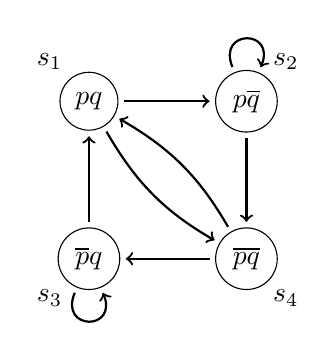
\begin{tikzpicture}
	[
	align=center,
	node/.style={circle,draw=black,fill=none},
	label/.style={draw=none,fill=none},
	arrow/.style={
           ->,
           thick,
           shorten <=2pt,
           shorten >=2pt,}
	]
		% nodes
		\node[node] (n1) at 		(-1.0,  1.0 ) {$p q$};
		\node[node] (n2) at 		( 1.0,  1.0 ) {$p \overline q$};
		\node[node] (n3) at 		(-1.0, -1.0 ) {$\overline p q$};
		\node[node] (n4) at 		( 1.0, -1.0 ) {$\overline p \overline q$};
		
		% labels
		\node[label] (l1) at 		(-1.5,  1.5 ) {$s_1$};
		\node[label] (l2) at 		( 1.5,  1.5 ) {$s_2$};
		\node[label] (l3) at 		(-1.5, -1.5 ) {$s_3$};
		\node[label] (l4) at 		( 1.5, -1.5 ) {$s_4$};
		
		% straight paths
		\foreach \from/\to in {n1/n2,n2/n4,n4/n3,n3/n1} \draw[arrow] (\from) -> (\to);
		
		% curved paths
		\draw[arrow] (n1) to [out=300,in=150,looseness=1] (n4);
		\draw[arrow] (n4) to [out=120,in=330,looseness=1] (n1);
		\draw[arrow] (n2) to [out=112.5,in=67.5,looseness=5] (n2);
		\draw[arrow] (n3) to [out=247.5,in=292.5,looseness=5] (n3);
		
	\end{tikzpicture}
	\label{fig:M_g-model}
	\caption{Model of ${\cal M}_g$}
\end{figure}

\newpage
\subsubsection*{(b) \mdseries Implement the model ${\cal M}_g$ in NuSMV with
all states as starting state. You may either use the 'stateful' or 'stateless'
approach (see first lecture on NuSMV).}
The code below translates all possibilities of movement along the paths of the
model ${\cal M}_g$ given.\footnote{Included with submission, see file
{\tt 5\_3b.smv} archived in {\tt code.zip}}
\begin{figure}[H]
	\lstinputlisting{M_g.smv}
	\label{code:M_g}
	\caption{NuSMV code of the ${\cal M}_g$ model}
\end{figure}

\section{Representation of Boolean formulas}
\subsection*{Question 6.3 \mdseries Recall that for any Boolean formula $f$,
\[ \forall x.f \eqdef f[0/x] \cdot f[1/x]
\quad \text{and} \quad
\exists x.f \eqdef f[0/x] + f[1/x] \]
Similar to these we can also define the {\it Boolean derivative} ($\partial$)
of $f$ (normally written as $\frac{\partial f}{\partial x}$, but we will here
use a shorter version) as
\[ \partial x.f \eqdef f[0/x] \oplus f[1/x] \]
Given the Boolean formula
\[ g = (x_1 x_2 x_3 + x_3 x_4) \oplus (x_2 + x_4 + x_1 x_3) \]
calculate the Boolean formula $\partial x_3.(\partial x_4.g)$. Simplify your
answer as much as possible. You must supply a line of reasoning, but you do
not need to convert into BDDs for this.}

First, we calculate the derivative $\partial x_4.g$; \footnote{I was unable to
find any definite answer on how to interpret when no operator is in-between
two boolean variables. I'm assuming that it is an implicit $\cdot$-operation
($\land$).}
\begin{align*}
	\partial x_4.g &=
	(x_1 x_2 x_3 + x_3 (0 \oplus 1))
	\oplus
	(x_2 + (0 \oplus 1) + x_1 x_3) \\
	&=
	(x_1 x_2 x_3 + x_3 1)
	\oplus
	(x_2 + 1 + x_1 x_3) \\
	&=
	(x_1 x_2 x_3 + x_3)
	\oplus 1
\end{align*}
And then we calculate derivate of $\partial x_3.(\partial x_4.g)$, by
substituting into the equation from the last calculated derivative;
\begin{align*}
	\partial x_3.(\partial x_4.g)
	&= \partial x_3.( (x_1 x_2 x_3 + x_3) \oplus 1 ) \\
	&= (x_1 x_2 (0 \oplus 1) + (0 \oplus 1) ) \oplus 1 \\
	&= (x_1 x_2 1 + 1) \oplus 1 \\
	&= 1 \oplus 1 \\
	&= 0
\end{align*}


\end{document}
